% On two occasions I have been asked, – "Pray, Mr. Babbage, if you put 
% into the machine wrong figures, will the right answers come out?" In 
% one case a member of the Upper, and in the other a member of the Lower
% House put this question. I am not able rightly to apprehend the kind
% of confusion of ideas that could provoke such a question.
% - Charles Babbage, Passages from the Life of a Philosopher (1864)
% (Ch. 5: "Difference Engine No. 1")

% (tn248)
% Created 7 Oct 2010
% At section 10 on 10 Oct 2010

% Because I keep forgetting: 
% In a terminal: R CMD Sweave filename.RnW
% In R: Sweave()

\documentclass[11pt, oneside, reqno]{article}
\usepackage{amssymb, amsthm, amsmath, amsfonts}

\usepackage{bardhw}
\usepackage{fullpage}
\usepackage[tableposition=top]{caption}
\usepackage{ifthen}
\usepackage{url}

% Euler for math | Palatino for rm | Helvetica for ss | Courier for tt
\renewcommand{\rmdefault}{ppl} % rm
\linespread{1.05}        % Palatino needs more leading
\usepackage[scaled]{helvet} % ss
\usepackage{courier} % tt
%\usepackage{euler} % math
\usepackage{eulervm} % a better implementation of the euler package (not in gwTeX)
\normalfont
\usepackage[T1]{fontenc}

\usepackage[utf8]{inputenc}


\usepackage{Sweave}
\begin{document}
	\setlength{\parindent}{0cm}
\normalfont
\setkeys{Gin}{width=3.5in}
\title{Scientific Programming Lab Exercises}
\date{}
%\author{Thomson Nguyen (tn248)}
\maketitle

\hwinfo{Thomson Nguyen (tn248)}{Scientific Programming (SP)}{\today}
\tableofcontents
\section{Interactive Calculations}

\url{http://www.cam.ac.uk}
\ans{Exercise 1.1}
These variable names \itshape{can't} be used:
\begin{itemize}
\item \verb@cell maximum size@ has spaces. Variables cannot contain blank spaces.

\item \verb@4min@ starts with a number. All variables must start with letters.

\item \verb@site#7@ contains a \#. All variables should contain alphanumeric characters.
\end{itemize}
\eans

\ans{Exercise 1.2}
The following values were computed in R:

\begin{enumerate}
\item  
\begin{Schunk}
\begin{Sinput}
> 2^7/(2^7 - 1)
\end{Sinput}
\begin{Soutput}
[1] 1.007874
\end{Soutput}
\end{Schunk}

\begin{Schunk}
\begin{Sinput}
> (1 - (1/2^7))^(-1)
\end{Sinput}
\begin{Soutput}
[1] 1.007874
\end{Soutput}
\end{Schunk}

\item
\begin{Schunk}
\begin{Sinput}
> sin(pi/9)
\end{Sinput}
\begin{Soutput}
[1] 0.3420201
\end{Soutput}
\end{Schunk}
\begin{Schunk}
\begin{Sinput}
> cos(pi/7)^2
\end{Sinput}
\begin{Soutput}
[1] 0.8117449
\end{Soutput}
\end{Schunk}

\item
\begin{Schunk}
\begin{Sinput}
> (2^7)/(2^7 - 1) + 4 * sin(pi/9)
\end{Sinput}
\begin{Soutput}
[1] 2.375955
\end{Soutput}
\end{Schunk}
\end{enumerate}
\eans

\ans{Exercise 1.3}
Apropos looks at the name of the function only, whilst help.search will find all instances of the string in its help pages.

\eans

\ans{Exercise 1.4}
Here is a histogram of 5000 random numbers with a Normal distribution:

\begin{Schunk}
\begin{Sinput}
> y = rnorm(5000)
> hist(y, breaks = 20)
\end{Sinput}
\end{Schunk}

\begin{figure}
\begin{center}
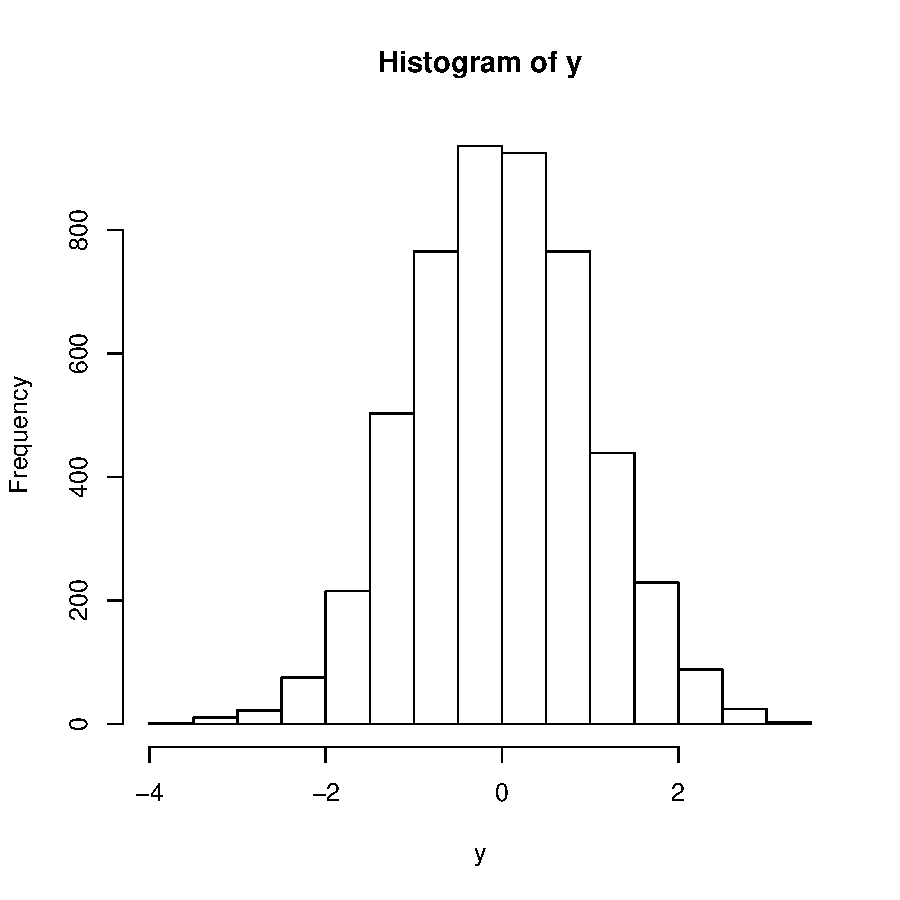
\includegraphics{exercises-fig1}
\end{center}
\caption{Histogram of 5000 random Normally distributed numbers.}
\label{fig:one}
\end{figure}

Setting the number of breaks in \verb@hist@ only suggests the number of bins. If you want a specific number of bins, you will have to create a vector with the bins specified (call it \verb@bins@)--then you would write:

\begin{Schunk}
\begin{Sinput}
> bins = seq(-5, 5, by = 0.5)
> hist(y, breaks = bins)
\end{Sinput}
\end{Schunk}
\eans

\section{An interactive section: fitting a linear regression model}

There were no exercises to answer in this section, but the example was fun.

\section{Script files and data files}

\ans{Exercise 3.1}
We were supposed to create a copy of \verb@Intro2.R@, and modify the copy so that the script performs linear regression of algal growth rate on the log of light intensity, and plots. This file is called \verb@Intro2Log.R@, and looks like this:

\begin{Schunk}
\begin{Sinput}
> X = read.table("ChlorellaGrowth.txt")
> X = as.matrix(X)
> Light = X[, 1]
> rmax = X[, 2]
> LogLight <- log(Light)
> par(cex = 1.5, cex.main = 0.9)
> xlabel = "Light intensity (uE/m2/s)"
> xlabelLog = "Log Light intensity (uE/m2/s)"
> ylabel = "Maximum growth rate rmax (1/d)"
> plot(LogLight, rmax, xlab = xlabel, ylab = ylabel, pch = 16)
> title(main = "Data from Fussmann et al. (2000) system")
> fitLog = lm(rmax ~ LogLight)
> abline(fitLog)
> c1Log = round(fitLog$coef[1], digits = 3)
> c2Log = round(fitLog$coef[2], digits = 3)
> text(3.8, 3, paste("rmax=", c1Log, "+", c2Log, "Log Light"))
\end{Sinput}
\end{Schunk}

This produces the following plot:

\begin{figure}
\begin{center}
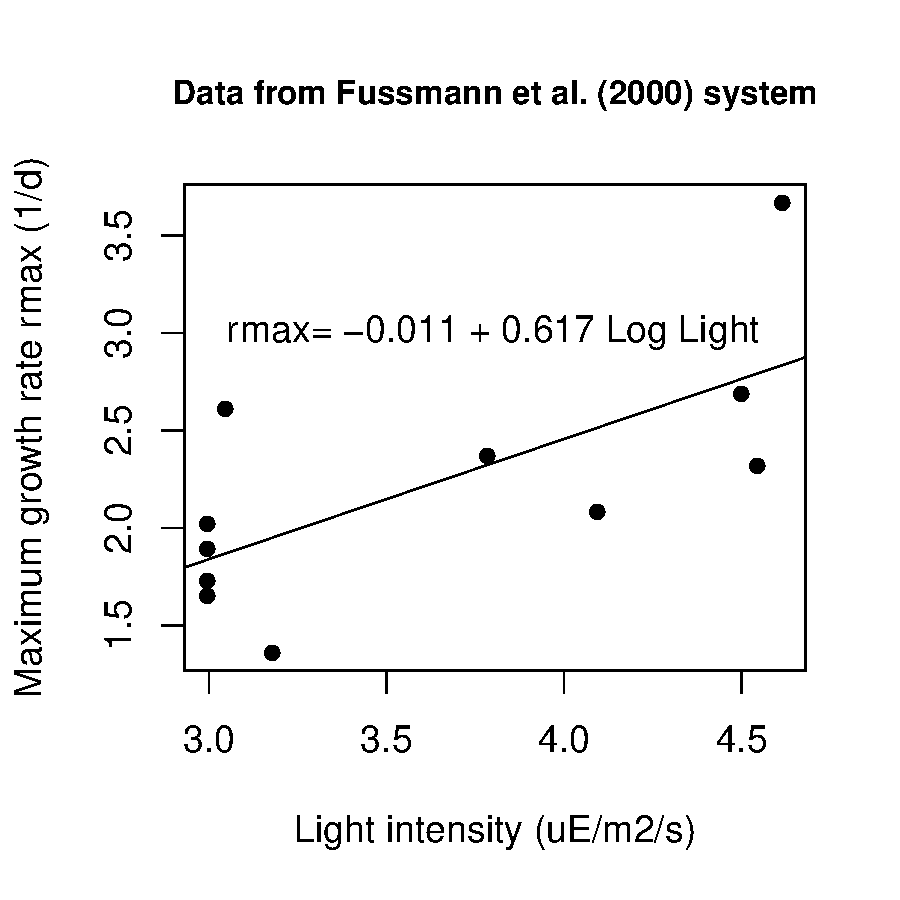
\includegraphics{exercises-fig2}
\end{center}
\caption{Regression Analysis of Log(Light).}
\label{fig:two}
\end{figure}
\eans

\ans{Exercise 3.2}
From the text: \emph{R produced a series of diagnostic plots exploring whether or not the fitter linear model is a suitable fit to the data. In each of the plots, the 3 most extreme points (the most likely candidates for "outliers") have been identified according to their sequence in the data set.}
\eans

\ans{Exercise 3.3}
The command to do so is:

\begin{Schunk}
\begin{Sinput}
> plot(Light, rmax, xlab = xlabel, ylab = ylabel, pch = 16, xlim = c(0, 
+     120), ylim = c(1, 4))
> fit = lm(rmax ~ Light)
> c1 = round(fit$coef[1], digits = 3)
> c2 = round(fit$coef[2], digits = 3)
> abline(fit)
> text(40, 3, paste("rmax=", c1, "+", c2, "Log Light"))
\end{Sinput}
\end{Schunk}

and it will generate a plot that looks like this:

\begin{figure}
\begin{center}
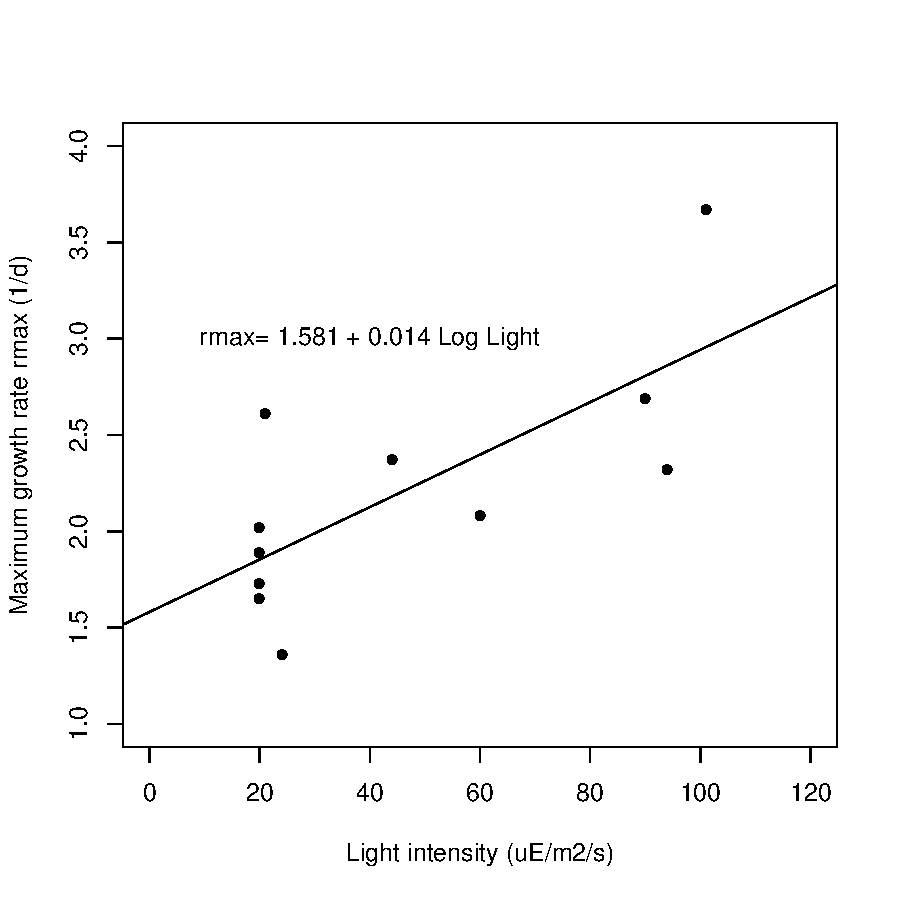
\includegraphics{exercises-fig3}
\end{center}
\caption{Regression Analysis of Light with updated axes.}
\label{fig:three}
\end{figure}
\eans

\ans{Exercise 3.4}
The following code block will plot both the linear and $\log$ plots as a single figure, in one column:

\begin{Schunk}
\begin{Sinput}
> par(mfcol = c(2, 1))
> plot(Light, rmax, xlab = xlabel, ylab = ylabel, pch = 16, xlim = c(0, 
+     120), ylim = c(1, 4))
> fit = lm(rmax ~ Light)
> abline(fit)
> text(40, 3, paste("rmax=", c1, "+", c2, "Light"))
> plot(LogLight, rmax, xlab = xlabelLog, ylab = ylabel, pch = 16)
> fit = lm(rmax ~ Light)
> abline(fitLog)
> text(3.8, 3, paste("rmax=", c1, "+", c2, "Log Light"))
\end{Sinput}
\end{Schunk}

\begin{figure}
\begin{center}
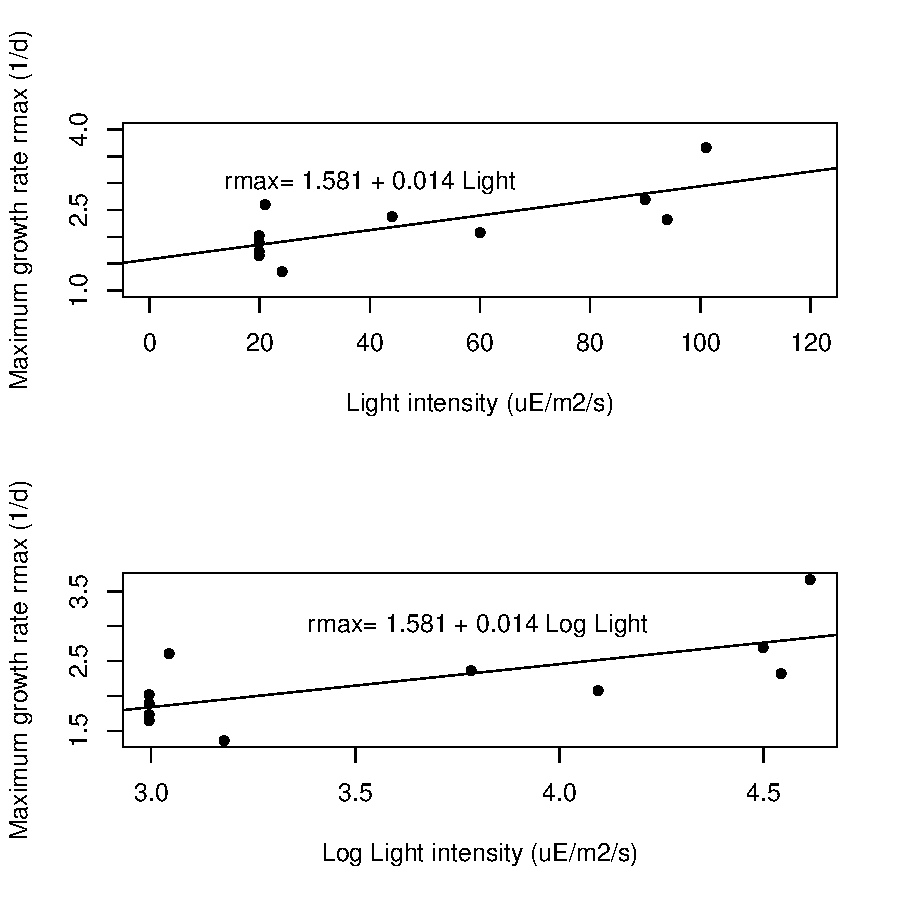
\includegraphics{exercises-LightOneColumn}
\end{center}
\caption{Regression Analysis of Light and $\log$ Light on one column.}
\label{fig:LightOneColumn}
\end{figure}

And the following code block will do the same thing, except in one row:

\begin{Schunk}
\begin{Sinput}
> par(mfcol = c(1, 2))
> plot(Light, rmax, xlab = xlabel, ylab = ylabel, pch = 16, xlim = c(0, 
+     120), ylim = c(1, 4))
> fit = lm(rmax ~ Light)
> abline(fit)
> text(40, 3, paste("rmax=", c1, "+", c2, "Light"))
> plot(LogLight, rmax, xlab = xlabelLog, ylab = ylabel, pch = 16)
> fit = lm(rmax ~ Light)
> abline(fitLog)
> text(3.8, 3, paste("rmax=", c1, "+", c2, "Log Light"))
\end{Sinput}
\end{Schunk}

\begin{figure}
\begin{center}
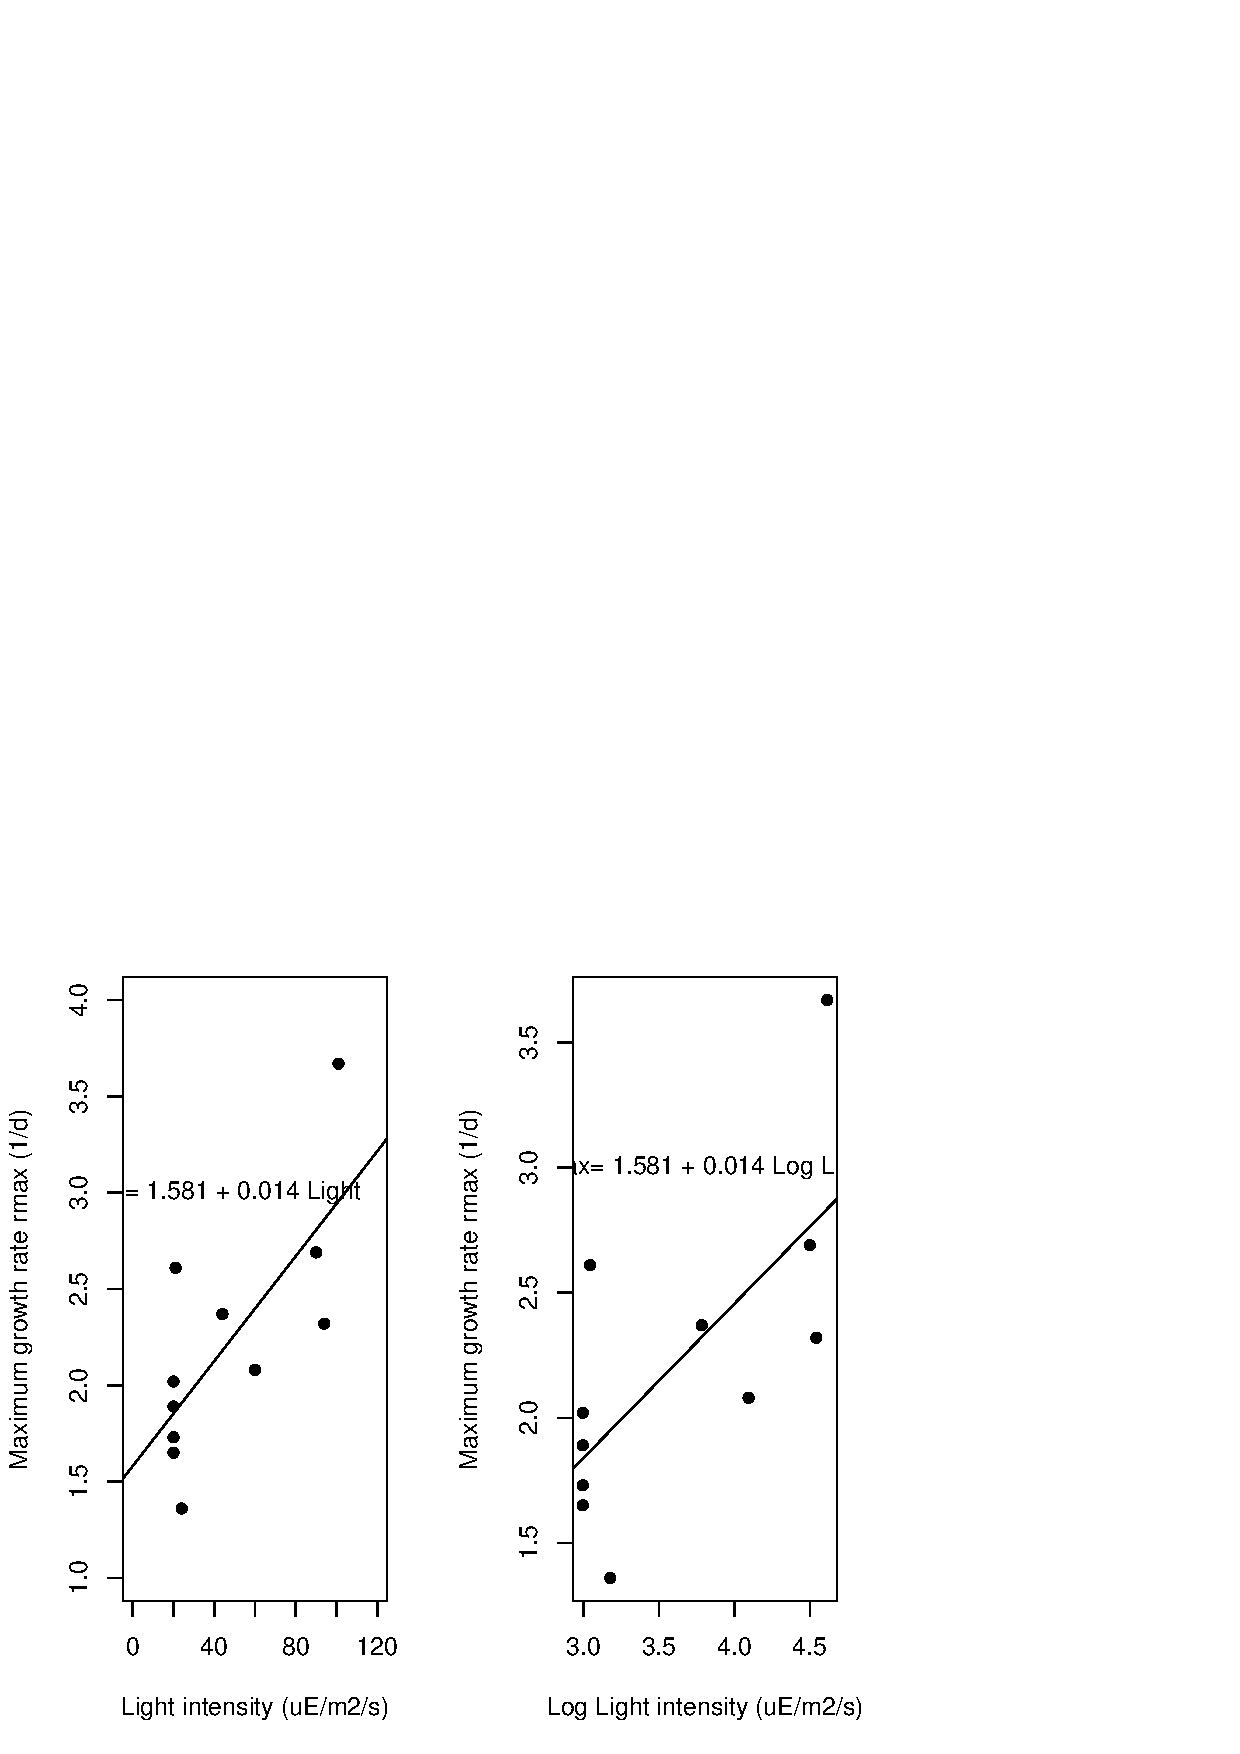
\includegraphics{exercises-LightOneRow}
\end{center}
\caption{Regression Analysis of Light and $\log$ Light on one Row.}
\label{fig:LightOneRow}
\end{figure}

\eans

\ans{Exercise 3.5}
The following code block will generate a $2\times 2$ set of plots, each showing the line $y=5x+3$ given $x\in [3,8]$, with four different line styles and colors:

\begin{Schunk}
\begin{Sinput}
> x <- 3:8
> y <- 5 * x + 3
> par(mfrow = c(2, 2))
> plot(x, y, pch = 10, col = "green")
> title(main = "Green blobs")
> plot(x, y, pch = 11, col = "red")
> title(main = "Red stars")
> plot(x, y, pch = 12, col = "black")
> title(main = "Black squares")
> plot(x, y, pch = 15, col = "blue")
> title(main = "Blue solid squares")
\end{Sinput}
\end{Schunk}

\begin{figure}
\begin{center}
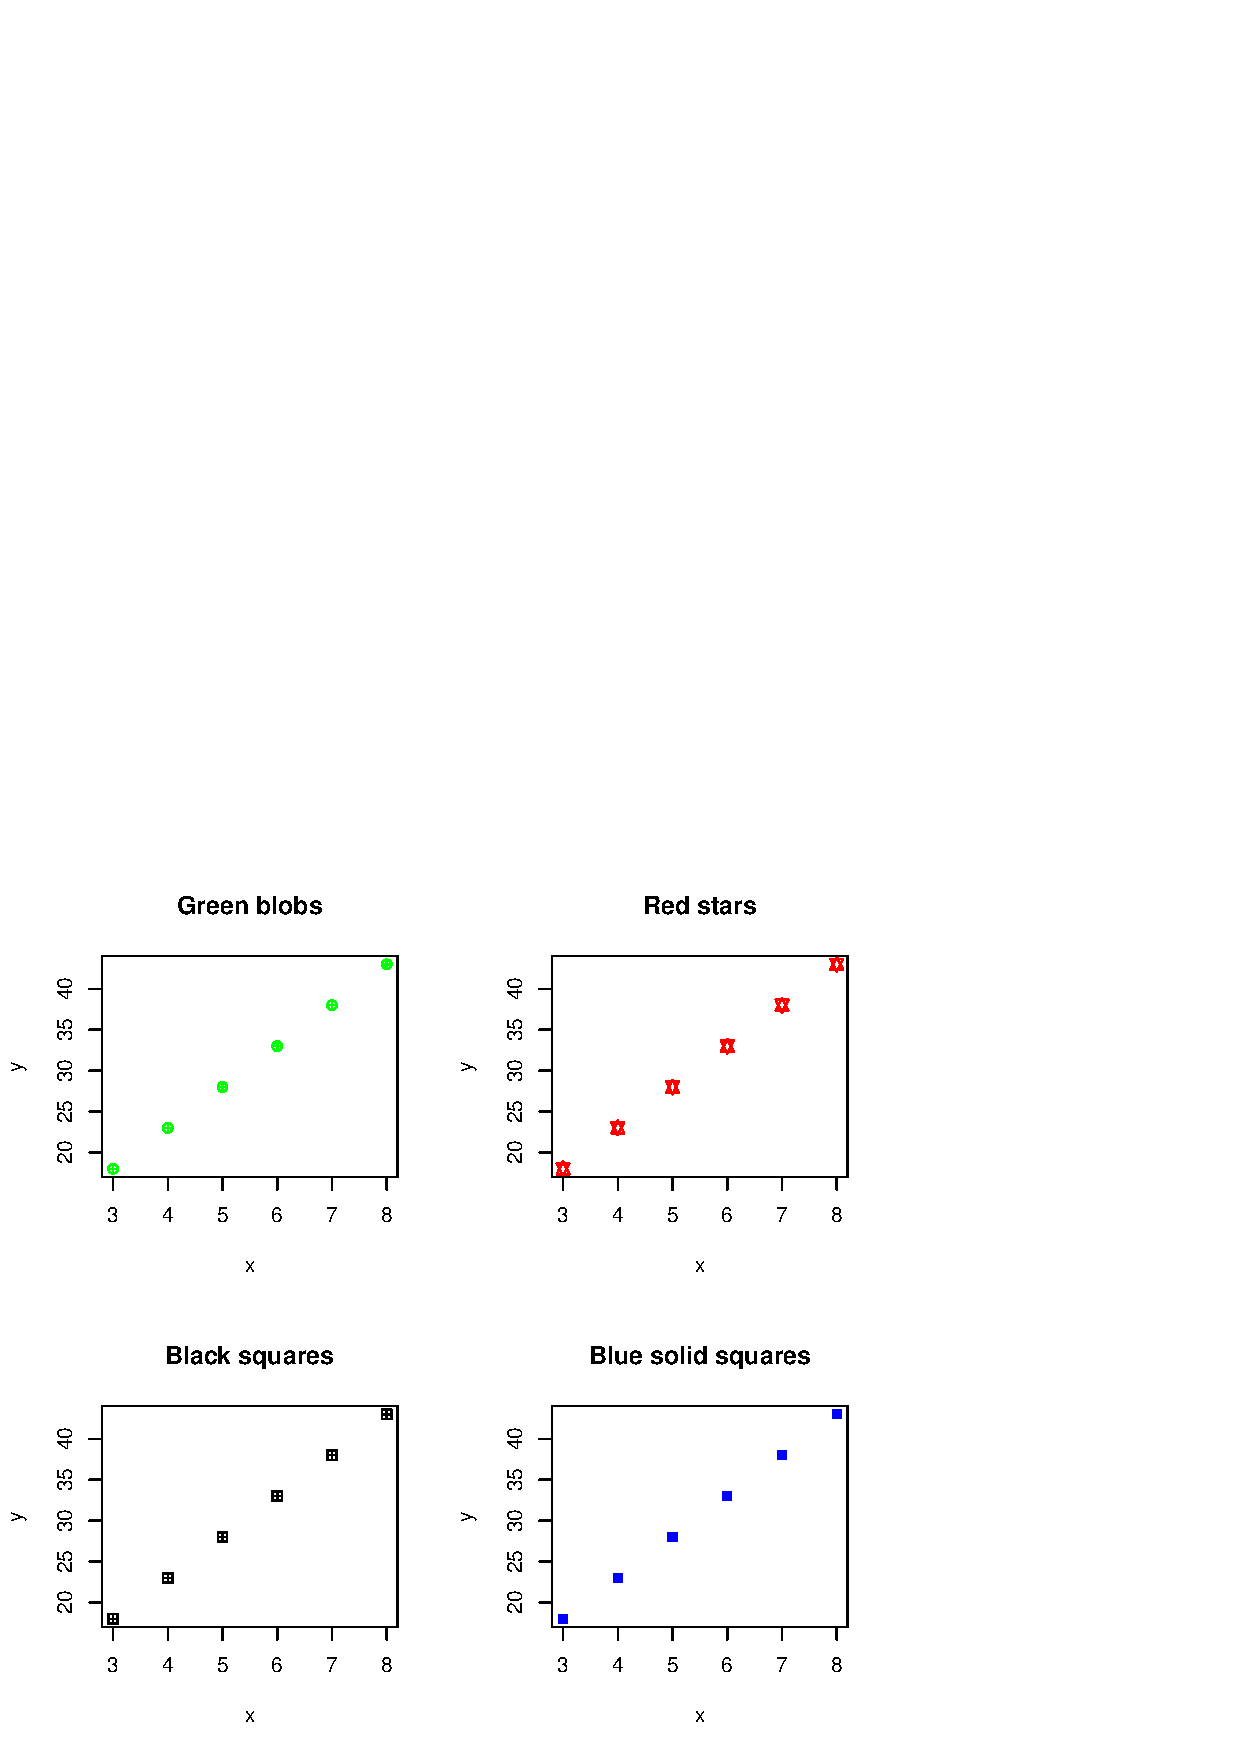
\includegraphics{exercises-twobytwo}
\end{center}
\caption{A $2\times 2$ set of plots of $y=5x+3$, with $x\in [3,8]$.}
\label{fig:twobytwo}
\end{figure}
\eans

\ans{Exercise 3.6}
If we want to save it to disk, we can use \verb@png()@, \verb@jpeg()@, \verb@pdf()@, or \verb@postscript()@ to prompt R to save it to disk. This example uses \verb@png()@.

\begin{Schunk}
\begin{Sinput}
> png("twobytwoplot.png")
> par(mfrow = c(2, 2))
> plot(x, y, pch = 10, col = "green")
> title(main = "Green blobs")
> plot(x, y, pch = 11, col = "red")
> title(main = "Red stars")
> plot(x, y, pch = 12, col = "black")
> title(main = "Black squares")
> plot(x, y, pch = 15, col = "blue")
> title(main = "Blue solid squares")
> dev.off()
\end{Sinput}
\begin{Soutput}
pdf 
  2 
\end{Soutput}
\end{Schunk}
\eans

\section{Vectors}

\ans{Exercise 4.1}

We want to create the vector \verb@v=(1 5 9 13)@ using \verb@seq@:
\begin{Schunk}
\begin{Sinput}
> v = seq(1, 13, length = 4)
> v
\end{Sinput}
\begin{Soutput}
[1]  1  5  9 13
\end{Soutput}
\end{Schunk}

Now we want to create a vector from $1$ to $5$ in increments of $0.2$, first with \verb@seq@, and then with some clever trickery of the form \verb@v=1+b*c(i:j)@:

\begin{Schunk}
\begin{Sinput}
> v1 = seq(1, 5, by = 0.2)
> v1
\end{Sinput}
\begin{Soutput}
 [1] 1.0 1.2 1.4 1.6 1.8 2.0 2.2 2.4 2.6 2.8 3.0 3.2 3.4 3.6 3.8 4.0 4.2 4.4 4.6
[20] 4.8 5.0
\end{Soutput}
\begin{Sinput}
> v2 = 1 + 0.2 * c(0:20)
> v2
\end{Sinput}
\begin{Soutput}
 [1] 1.0 1.2 1.4 1.6 1.8 2.0 2.2 2.4 2.6 2.8 3.0 3.2 3.4 3.6 3.8 4.0 4.2 4.4 4.6
[20] 4.8 5.0
\end{Soutput}
\begin{Sinput}
> v1 == v2
\end{Sinput}
\begin{Soutput}
 [1] TRUE TRUE TRUE TRUE TRUE TRUE TRUE TRUE TRUE TRUE TRUE TRUE TRUE TRUE TRUE
[16] TRUE TRUE TRUE TRUE TRUE TRUE
\end{Soutput}
\end{Schunk}
\eans

\ans{Exercise 4.2}
We want to create a vector of 5000 normally distributed random numbers with mean=3, standard deviation=2:

\begin{Schunk}
\begin{Sinput}
> v = rnorm(5000, mean = 3, sd = 2)
> mean(v)
\end{Sinput}
\begin{Soutput}
[1] 3.042928
\end{Soutput}
\begin{Sinput}
> sd(v)
\end{Sinput}
\begin{Soutput}
[1] 1.960032
\end{Soutput}
\end{Schunk}

\begin{Schunk}
\begin{Sinput}
> hist(v, breaks = 20)
\end{Sinput}
\end{Schunk}

\begin{figure}
\begin{center}
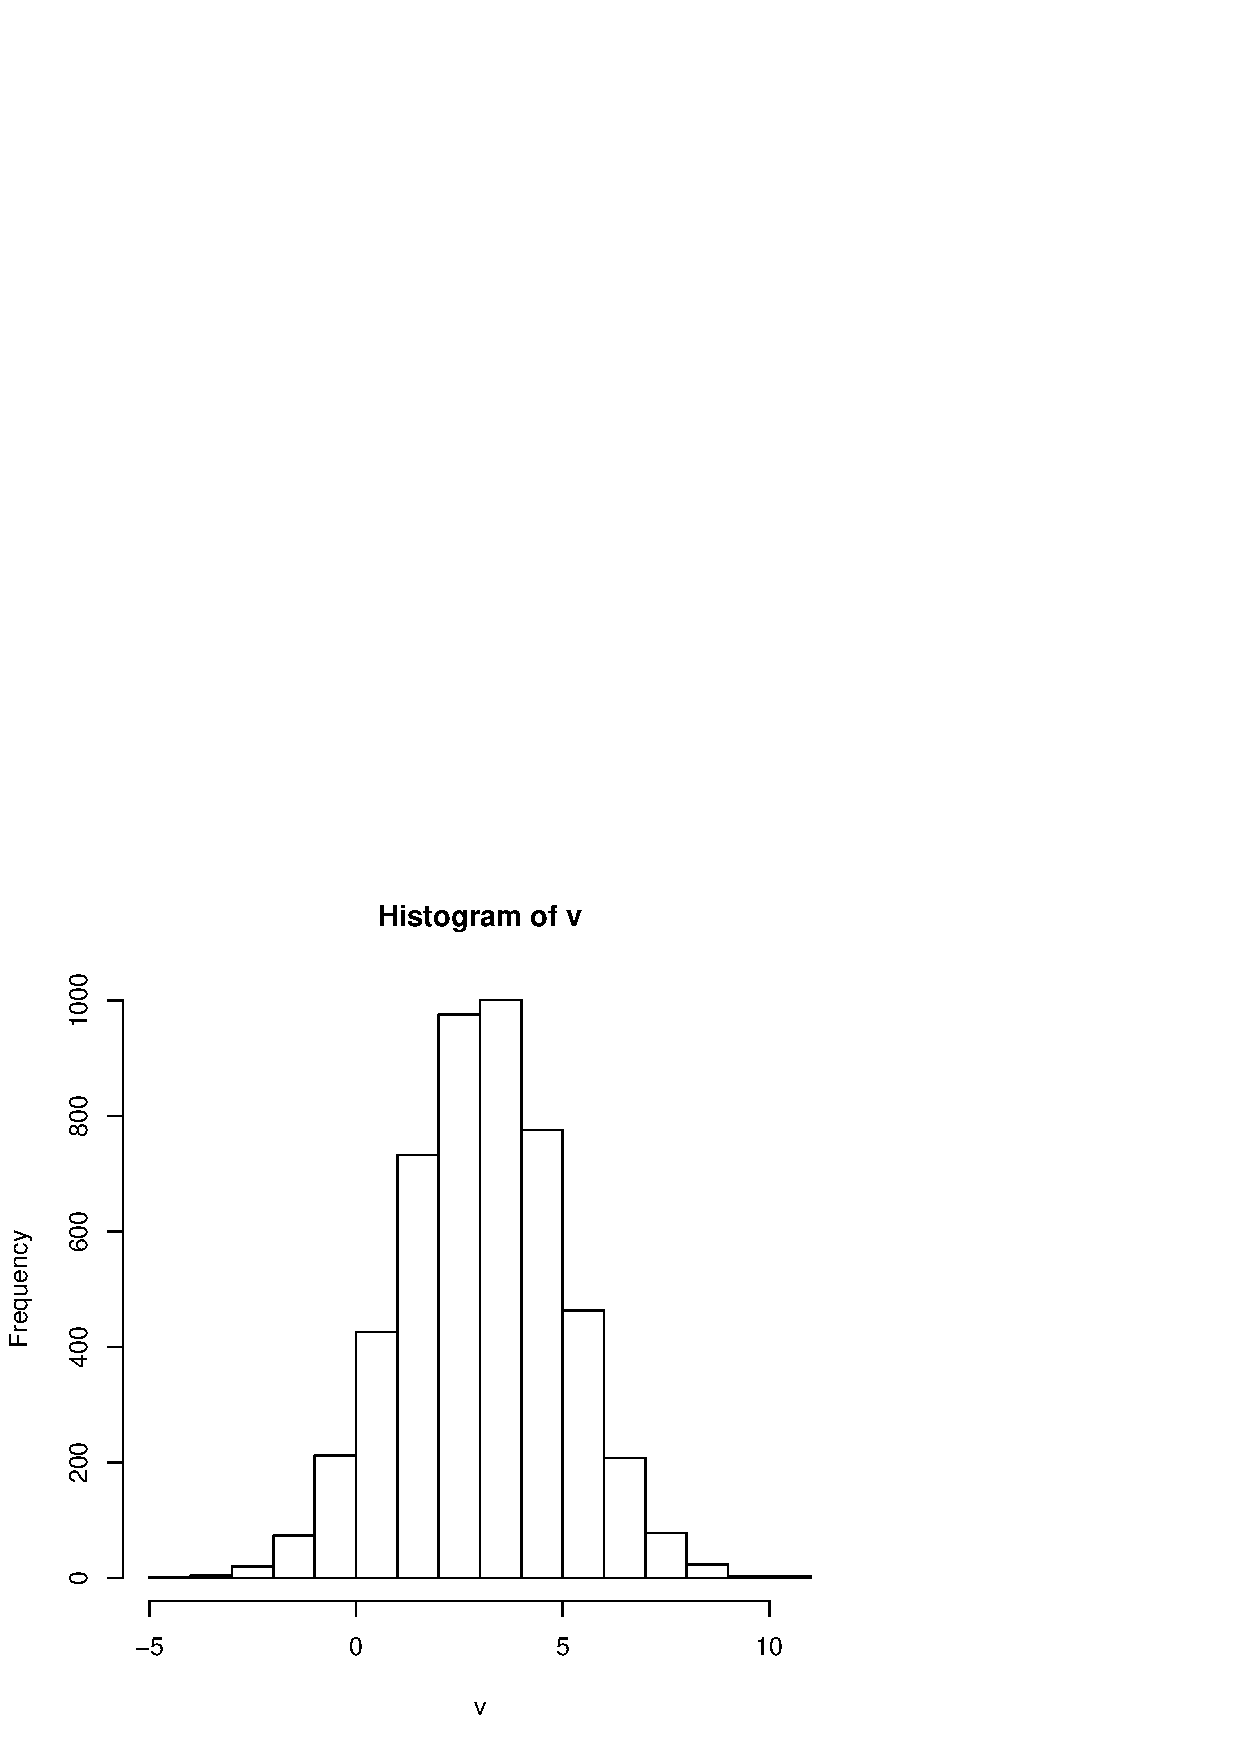
\includegraphics{exercises-fivethousandrnorm}
\end{center}
\caption{Histogram of 5000 normally distributed numbers with $\bar{x}=3$, $\sigma=2$.}
\label{fig:fivethousand}
\end{figure}
\eans

\ans{Exercise 4.3}
We are to create a finite geometric series $1+r+r^2+\ldots+r^n$ with $r=0.5$ and $n=10$, and compute its sum:

\begin{Schunk}
\begin{Sinput}
> 1 + sum(0.5^c(1:10))
\end{Sinput}
\begin{Soutput}
[1] 1.999023
\end{Soutput}
\end{Schunk}

Compare this to the limiting value for any geometric series:

\[
\frac{1}{1-r}
\]

\begin{Schunk}
\begin{Sinput}
> 1/(1 - 0.5)
\end{Sinput}
\begin{Soutput}
[1] 2
\end{Soutput}
\end{Schunk}

and you can see we're a bit off. We increase accuracy by increasing the resolution:

\begin{Schunk}
\begin{Sinput}
> 1 + sum(0.5^c(1:50))
\end{Sinput}
\begin{Soutput}
[1] 2
\end{Soutput}
\begin{Sinput}
> 1 + sum(0.5^c(1:5000))
\end{Sinput}
\begin{Soutput}
[1] 2
\end{Soutput}
\end{Schunk}

GO BACK TO THIS ONE
\eans

\ans{Exercise 4.4}
Given \verb@q = c(1,3,5,7,9,11)@, we want to extract the second, first, and third elements of \verb@q@ in that order:

\begin{Schunk}
\begin{Sinput}
> q = c(1, 3, 5, 7, 9, 11)
> q[c(2, 1, 3)]
\end{Sinput}
\begin{Soutput}
[1] 3 1 5
\end{Soutput}
\end{Schunk}

\eans

\ans{Exercise 4.5}
We want to write a script that computes values of $z=\frac{(x-1)}{(x+1)}$ and $w=\frac{\sin(x^2)}{x^2}$ for $x=1,2,\ldots,12$ and plots both of these functions of x with points connected by a line:


\begin{Schunk}
\begin{Sinput}
> x = c(1:12)
> z = (x - 1)/(x + 1)
> w = (sin(x^2)/x^2)
\end{Sinput}
\end{Schunk}

\begin{Schunk}
\begin{Sinput}
> plot(x, z, col = "red", type = "o", lty = 1, pch = 22, ylim = c(-0.4, 
+     1))
> lines(x, w, col = "blue", type = "o", lty = 1, pch = 22)
> legend(2, 1, c("z(x)", "w(x)"), cex = 0.8, col = c("red", "blue"), 
+     pch = 22, lty = 1)
\end{Sinput}
\end{Schunk}

\begin{figure}
\begin{center}
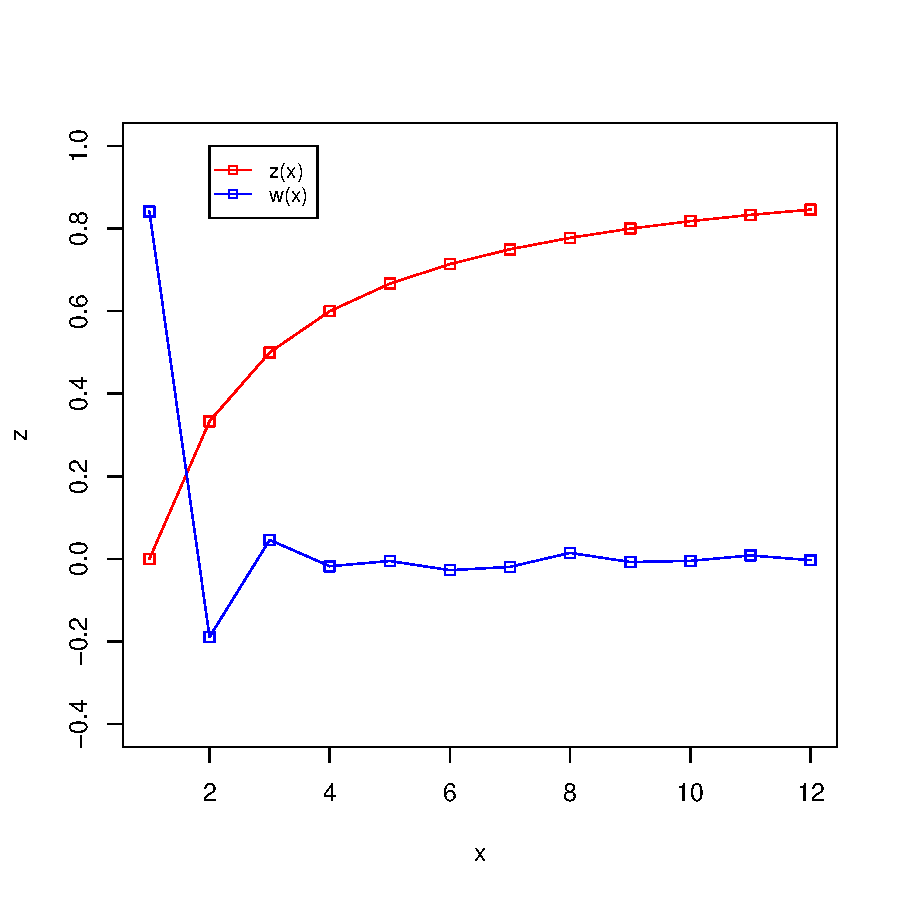
\includegraphics{exercises-twoplots}
\end{center}
\caption{Plots of $z(x)$ and $w(x)$.}
\label{fig:twoplots}
\end{figure}

\eans

\section{Matrices}

\ans{Exercise 5.1}
Here, we're going to create the following matrix in R:
\[
\begin{pmatrix}
1&1&1&1\\
2&2&2&2
\end{pmatrix}
\]

\begin{Schunk}
\begin{Sinput}
> X = matrix(c(rep(1, 4), rep(2, 4)), 2, 4)
> X
\end{Sinput}
\begin{Soutput}
     [,1] [,2] [,3] [,4]
[1,]    1    1    2    2
[2,]    1    1    2    2
\end{Soutput}
\end{Schunk}

\eans

\ans{Exercise 5.2}
Here, we're going to use \verb@rnorm@ and \verb@matrix@ to create a $5\times 7$ matrix of Gaussian random numbers with mean $1$ and standard deviation 2:

\begin{Schunk}
\begin{Sinput}
> matrix(rnorm(35, mean = 1, sd = 2), 5, 7)
\end{Sinput}
\begin{Soutput}
          [,1]       [,2]      [,3]      [,4]      [,5]        [,6]       [,7]
[1,] 3.4984620  3.0307887 -1.404281 0.7701578 2.3315037 -1.87928639  0.1214449
[2,] 0.6407679  0.6037209  1.134974 2.9329151 1.8892535  0.09193704  2.3681593
[3,] 0.5456423 -0.9752852  2.285530 0.6615644 0.3332494  1.58000836 -0.6587874
[4,] 0.6055490  2.1593517  1.401210 1.7761304 4.6690506 -2.35115581  0.8102160
[5,] 3.0107823  0.5853313  3.069421 2.3223055 2.1924174  3.36680297  2.4053006
\end{Soutput}
\end{Schunk}

\eans

\ans{Exercise 5.3}

If we have $A$ and $B$ defined as follows:

\begin{Schunk}
\begin{Sinput}
> A = cbind(1:3, 4:6, 7:9)
> A
\end{Sinput}
\begin{Soutput}
     [,1] [,2] [,3]
[1,]    1    4    7
[2,]    2    5    8
[3,]    3    6    9
\end{Soutput}
\begin{Sinput}
> B = rbind(1:3, 4:6)
> B
\end{Sinput}
\begin{Soutput}
     [,1] [,2] [,3]
[1,]    1    2    3
[2,]    4    5    6
\end{Soutput}
\end{Schunk}

and we want to combine the two matrices together, we'll see that

\begin{Schunk}
\begin{Sinput}
> rbind(A, B)
\end{Sinput}
\begin{Soutput}
     [,1] [,2] [,3]
[1,]    1    4    7
[2,]    2    5    8
[3,]    3    6    9
[4,]    1    2    3
[5,]    4    5    6
\end{Soutput}
\begin{Sinput}
> cbind(A, A)
\end{Sinput}
\begin{Soutput}
     [,1] [,2] [,3] [,4] [,5] [,6]
[1,]    1    4    7    1    4    7
[2,]    2    5    8    2    5    8
[3,]    3    6    9    3    6    9
\end{Soutput}
\end{Schunk}

both work,but \verb@cbind(A,B)@ won't. This is because the number of rows in $A$ and $B$ differ. 

\eans

\ans{Exercise 5.4}
With \verb@runif@ we can create a $5\times 5$ matrix of random numbers with a uniform distribution between $0$ and $1$:

\begin{Schunk}
\begin{Sinput}
> B = matrix(runif(25), 5, 5)
> B
\end{Sinput}
\begin{Soutput}
          [,1]      [,2]       [,3]        [,4]       [,5]
[1,] 0.9947380 0.3392569 0.66120471 0.006922941 0.56995343
[2,] 0.1593925 0.6527678 0.29688099 0.827556818 0.30316369
[3,] 0.4816927 0.8187656 0.85456175 0.431427286 0.18807422
[4,] 0.2491387 0.3973978 0.02986787 0.619128408 0.06134062
[5,] 0.5086294 0.1190234 0.13815354 0.305004088 0.83995365
\end{Soutput}
\begin{Sinput}
> B[2, ]
\end{Sinput}
\begin{Soutput}
[1] 0.1593925 0.6527678 0.2968810 0.8275568 0.3031637
\end{Soutput}
\begin{Sinput}
> B[, 2]
\end{Sinput}
\begin{Soutput}
[1] 0.3392569 0.6527678 0.8187656 0.3973978 0.1190234
\end{Soutput}
\begin{Sinput}
> B[2:4, 2:4]
\end{Sinput}
\begin{Soutput}
          [,1]       [,2]      [,3]
[1,] 0.6527678 0.29688099 0.8275568
[2,] 0.8187656 0.85456175 0.4314273
[3,] 0.3973978 0.02986787 0.6191284
\end{Soutput}
\begin{Sinput}
> B[1, ] = seq(2, 14, by = 3)
> B
\end{Sinput}
\begin{Soutput}
          [,1]      [,2]       [,3]       [,4]        [,5]
[1,] 2.0000000 5.0000000 8.00000000 11.0000000 14.00000000
[2,] 0.1593925 0.6527678 0.29688099  0.8275568  0.30316369
[3,] 0.4816927 0.8187656 0.85456175  0.4314273  0.18807422
[4,] 0.2491387 0.3973978 0.02986787  0.6191284  0.06134062
[5,] 0.5086294 0.1190234 0.13815354  0.3050041  0.83995365
\end{Soutput}
\end{Schunk}

\eans

\section{Iteration (``Looping")}

\ans{Exercise 6.1}
At $t=0$, I have $400$ parasites and my assistant has $120$. I, however, accumulate additional parasites at a rate of $10\%$ every day, whilst my assistant accumulates at the increased rate of $20\%$. We model this with following two equations, where $t$ is the number of days after returning:

\begin{align*}
n(t)&=400(1.1)^t\\
m(t)&=120(1.2)^t,
\end{align*}

where $n$ is me, and $m$ is my assistant. 

Our script file \verb@Parasite1.R@ will use a for-loop to compute the number of parasites in both bodies over 30 days, and plot both log(parasites) versus time:

\begin{Schunk}
\begin{Sinput}
> n = rep(0, 31)
> m = rep(0, 31)
> t = c(0:30)
> for (i in t) {
+     n[i + 1] = 400 * (1.1)^i
+     m[i + 1] = 120 * (1.2)^i
+ }
\end{Sinput}
\end{Schunk}

\begin{Schunk}
\begin{Sinput}
> plot(t, log(n), col = "black", type = "o", lty = 1, pch = 20, 
+     ylab = "Number of parasites", xlab = "Time (in days)", ylim = c(4.5, 
+         10.2))
> lines(t, log(m), col = "red", type = "o", lty = 1, pch = 20)
> legend(2, 10, c("Me", "My assistant"), cex = 0.8, col = c("black", 
+     "red"), pch = 20, lty = 1)
\end{Sinput}
\end{Schunk}

\begin{figure}
\begin{center}
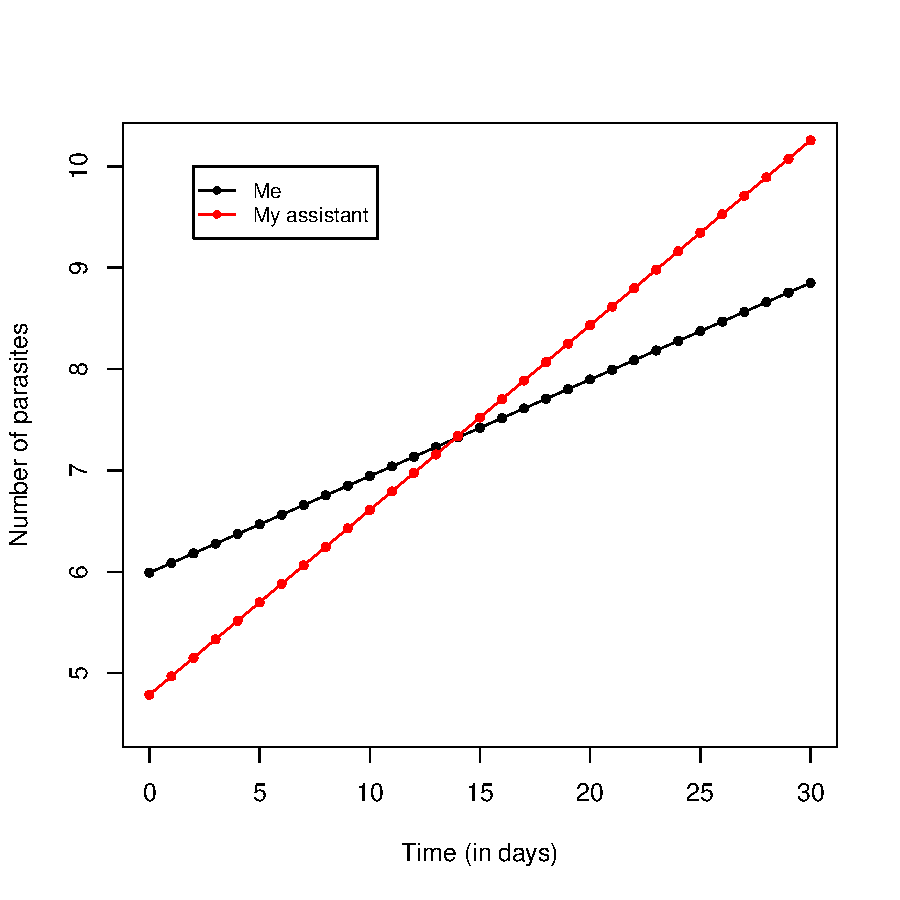
\includegraphics{exercises-disease}
\end{center}
\caption{Plot of a nasty parasite spreading through me and my assistant over 30 days.}
\label{fig:disease}
\end{figure}

\eans


\ans{Exercise 6.2}

We will now construct the following $5\times 5$ matrix (call it $A$) using a nested for-loop\footnote{There is definitely a better way to do this.}:

\[
\begin{pmatrix}
0&1&2&3&4\\
0.1&0&0&0&0\\
0&0.2&0&0&0\\
0&0&0.3&0&0\\
0&0&0&0.4&0
\end{pmatrix}
\]


\begin{Schunk}
\begin{Sinput}
> A = matrix(0, 5, 5)
> for (row in 1:5) {
+     if (row == 1) {
+         for (col in 1:5) {
+             A[row, col] = col - row
+         }
+     }
+     else {
+         for (col in 1:5) {
+             if (row == col + 1) 
+                 A[row, col] = col/10
+         }
+     }
+ }
> A
\end{Sinput}
\begin{Soutput}
     [,1] [,2] [,3] [,4] [,5]
[1,]  0.0  1.0  2.0  3.0    4
[2,]  0.1  0.0  0.0  0.0    0
[3,]  0.0  0.2  0.0  0.0    0
[4,]  0.0  0.0  0.3  0.0    0
[5,]  0.0  0.0  0.0  0.4    0
\end{Soutput}
\end{Schunk}

\eans

\ans{Exercise 6.3}
We will now rewrite \verb@Parasite1.R@ (see Exercise 6.1) to terminate when my assistant is sicker. Call this new script \verb@Parasite2.R@:

\begin{Schunk}
\begin{Sinput}
> n = 400
> m = 120
> t = 1
> while (n[t] > m[t]) {
+     n[t + 1] = 400 * (1.1)^t
+     m[t + 1] = 120 * (1.2)^t
+     t <- t + 1
+ }
> n
\end{Sinput}
\begin{Soutput}
 [1]  400.0000  440.0000  484.0000  532.4000  585.6400  644.2040  708.6244
 [8]  779.4868  857.4355  943.1791 1037.4970 1141.2467 1255.3714 1380.9085
[15] 1518.9993
\end{Soutput}
\begin{Sinput}
> m
\end{Sinput}
\begin{Soutput}
 [1]  120.0000  144.0000  172.8000  207.3600  248.8320  298.5984  358.3181
 [8]  429.9817  515.9780  619.1736  743.0084  891.6100 1069.9321 1283.9185
[15] 1540.7022
\end{Soutput}
\end{Schunk}

We see that day 15 is the day my assistant becomes sicker.
\eans

\ans{Exercise 6.4}
We want to use \verb@identical@ to determine whether all entries in an \verb@rnorm(5)@ are positive:
\begin{Schunk}
\begin{Sinput}
> a = rnorm(5)
> a
\end{Sinput}
\begin{Soutput}
[1] -0.6854255  1.0315123 -1.4192830 -1.1942154 -0.1778668
\end{Soutput}
\begin{Sinput}
> identical(a > 0, rep(TRUE, 5))
\end{Sinput}
\begin{Soutput}
[1] FALSE
\end{Soutput}
\end{Schunk}
\eans

\section{Branching}

\ans{Exercise 7.1}
There wasn't really an exercise here more than there was a call to check out the following script \verb@Branch.R@:

\begin{Schunk}
\begin{Sinput}
> initsize = 10
> popsize = initsize
> popnow = initsize
> while (popnow < 1000) {
+     if (popnow < 250) {
+         popnow = popnow * 2
+     }
+     else {
+         popnow = popnow * 1.5
+     }
+     popsize = c(popsize, popnow)
+ }
> tvals = 1:length(popsize)
> plot(tvals, log(popsize), type = "o", col = "red", xlab = "Generation", 
+     ylab = "Population size", pch = 16, cex = 1.25)
> title(main = "Geometric growth model")
\end{Sinput}
\end{Schunk}
\eans

\ans{Exercise 7.2}
We're now going to modify \verb@Parasite1.R@ so that there is random variation in parasite reproduction:

\begin{Schunk}
\begin{Sinput}
> n = 400
> m = 120
> t = c(1:29)
> for (i in t) {
+     if (runif(1) < 0.5) {
+         n[i + 1] = n[i] * (0.9)
+         m[i + 1] = m[i] * (0.8)
+     }
+     else {
+         n[i + 1] = n[i] * (1.1)
+         m[i + 1] = m[i] * (1.2)
+     }
+ }
\end{Sinput}
\end{Schunk}

\begin{Schunk}
\begin{Sinput}
> plot(c(t, 30), n, col = "black", type = "o", lty = 1, pch = 20, 
+     ylab = "Number of parasites", xlab = "Time (in days)", ylim = c(min(min(n), 
+         min(m)), max(max(n), max(m))))
> lines(c(t, 30), m, col = "red", type = "o", lty = 1, pch = 20)
> legend(2, max(max(n), max(m)), c("Me", "My assistant"), cex = 0.8, 
+     col = c("black", "red"), pch = 20, lty = 1)
\end{Sinput}
\end{Schunk}

\begin{figure}
\begin{center}
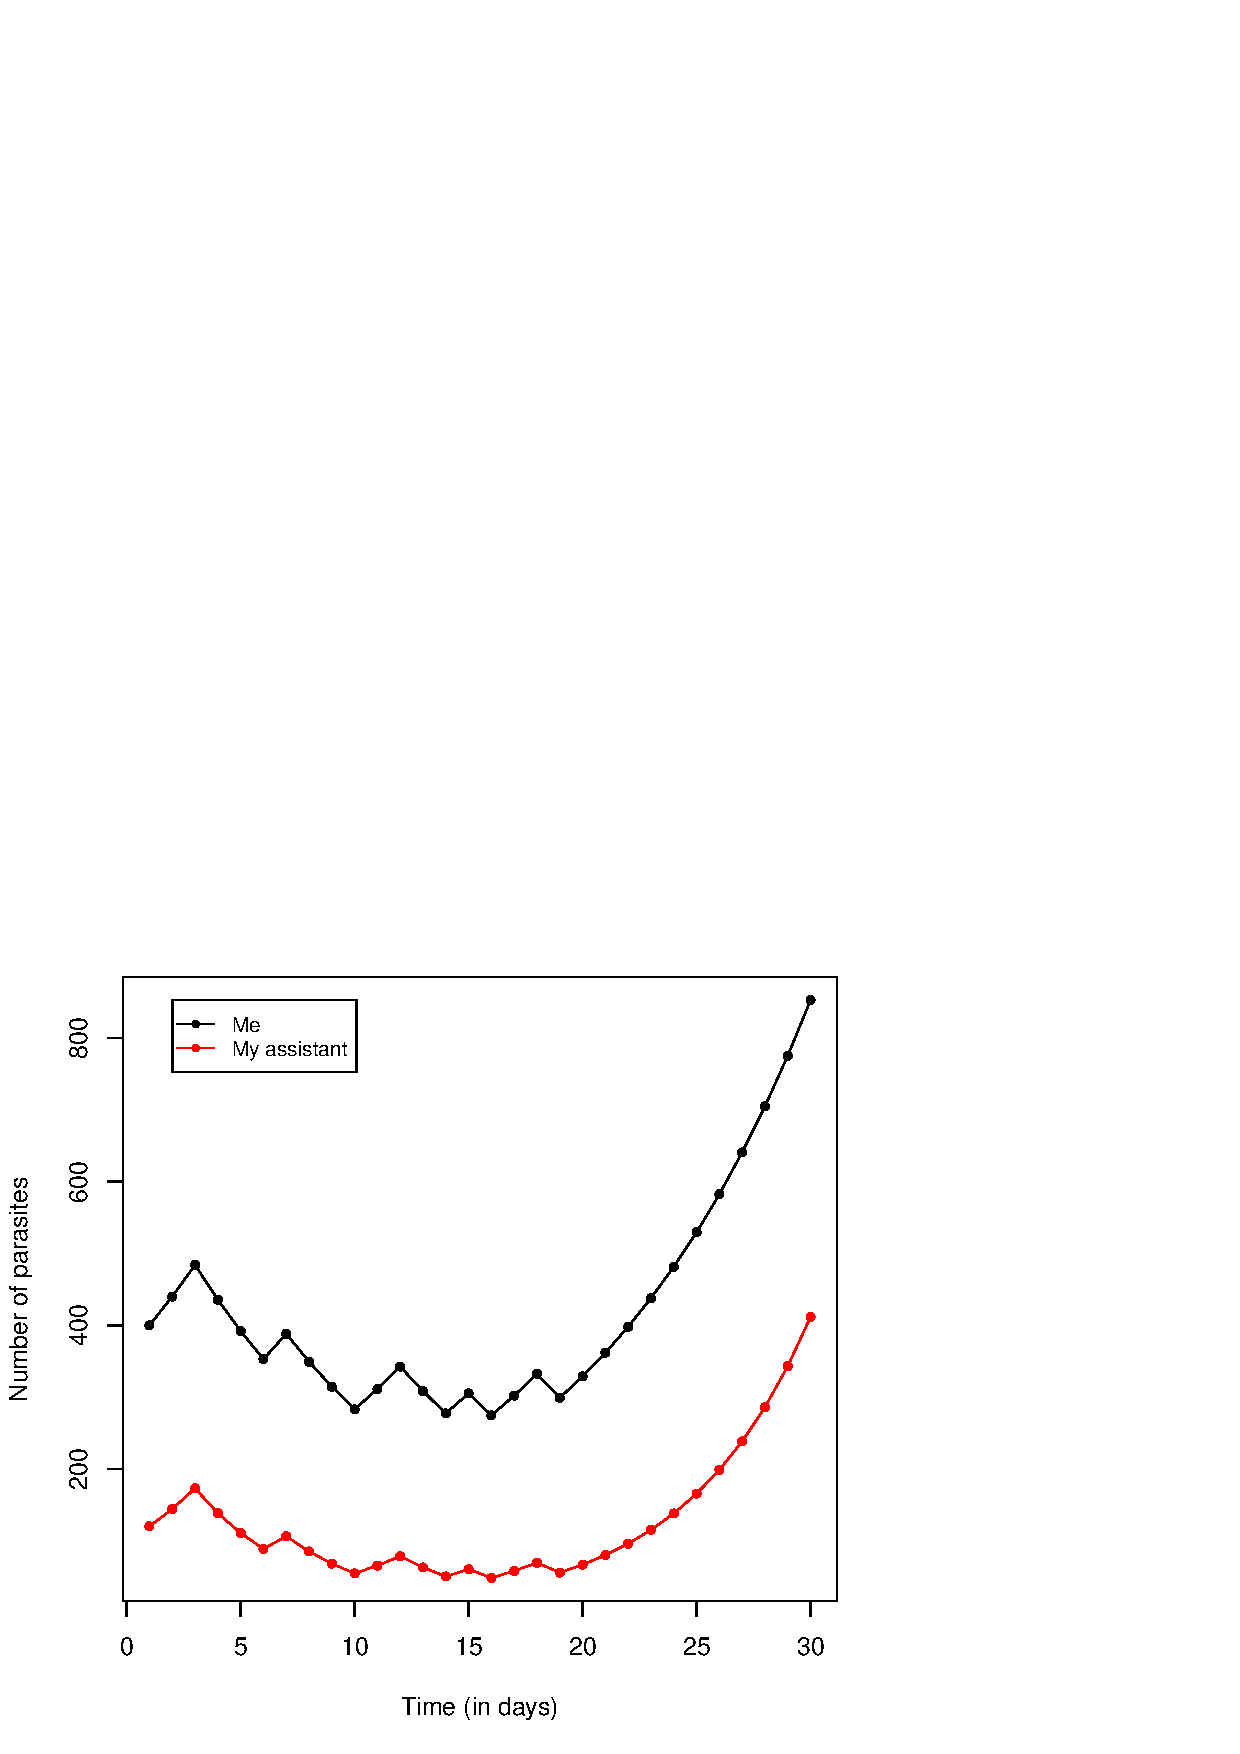
\includegraphics{exercises-diseasevar}
\end{center}
\caption{Plot of a nasty parasite spreading through me and my assistant over 30 days, with the variation coin-flip.}
\label{fig:diseasevar}
\end{figure}
\eans

\section{Numerical Matrix Algebra}
\ans{Exercise 8.1}
We can find the eigenvalues of a matrix as follows:
\begin{Schunk}
\begin{Sinput}
> A = matrix(1:9, 3, 3)
> vA = eigen(A)
> vA
\end{Sinput}
\begin{Soutput}
$values
[1]  1.611684e+01 -1.116844e+00 -5.113824e-16

$vectors
           [,1]       [,2]       [,3]
[1,] -0.4645473 -0.8829060  0.4082483
[2,] -0.5707955 -0.2395204 -0.8164966
[3,] -0.6770438  0.4038651  0.4082483
\end{Soutput}
\begin{Sinput}
> j = 1
> A %*% vA$vectors[, j] - vA$values[j] * vA$vectors[, j]
\end{Sinput}
\begin{Soutput}
             [,1]
[1,] 8.881784e-16
[2,] 1.776357e-15
[3,] 1.065814e-14
\end{Soutput}
\begin{Sinput}
> j = 2
> A %*% vA$vectors[, j] - vA$values[j] * vA$vectors[, j]
\end{Sinput}
\begin{Soutput}
             [,1]
[1,] 3.108624e-15
[2,] 4.829470e-15
[3,] 5.384582e-15
\end{Soutput}
\begin{Sinput}
> j = 3
> A %*% vA$vectors[, j] - vA$values[j] * vA$vectors[, j]
\end{Sinput}
\begin{Soutput}
              [,1]
[1,] -1.567586e-15
[2,] -2.637988e-15
[3,] -2.455764e-15
\end{Soutput}
\end{Schunk}

What we are seeing here is the following identity:

\[
Ax - \lambda I x = 0;
\]

however, there is some numerical roundoff error present. 
\eans

\ans{Exercise 8.2}
The \verb@names@ command will return the names of an object, like so:

\begin{Schunk}
\begin{Sinput}
> names(vA)
\end{Sinput}
\begin{Soutput}
[1] "values"  "vectors"
\end{Soutput}
\end{Schunk}

If we have an object with no names, or if the object can't have any names, it'll return a \verb@NULL@:

\begin{Schunk}
\begin{Sinput}
> names(A)
\end{Sinput}
\begin{Soutput}
NULL
\end{Soutput}
\end{Schunk}

\eans

\ans{Exercise 8.3}
We can find the left eigenvalues of $A$ as follows:

\begin{Schunk}
\begin{Sinput}
> vLA = eigen(t(A))$vectors
> j = 1
> vLA[, j] %*% A - vA$values[j] * vLA[, j]
\end{Sinput}
\begin{Soutput}
             [,1]         [,2]         [,3]
[1,] 7.993606e-15 3.552714e-15 7.105427e-15
\end{Soutput}
\begin{Sinput}
> j = 2
> vLA[, j] %*% A - vA$values[j] * vLA[, j]
\end{Sinput}
\begin{Soutput}
              [,1]          [,2]          [,3]
[1,] -8.881784e-16 -1.332268e-15 -2.664535e-15
\end{Soutput}
\begin{Sinput}
> j = 3
> vLA[, j] %*% A - vA$values[j] * vLA[, j]
\end{Sinput}
\begin{Soutput}
              [,1]          [,2]          [,3]
[1,] -6.794074e-16 -1.305720e-15 -1.123497e-15
\end{Soutput}
\end{Schunk}

\eans

\ans{Exercise 8.4}
We want to find all the eigenvalues for the following matrices:

\[
A= 
\begin{pmatrix}
	1&-5&0\\6&4&0\\0&0&2
\end{pmatrix}
\qquad
B=
\begin{pmatrix}
	0&1&5\\0.6&0&0\\0&0.4&0.9
\end{pmatrix}
\]


\begin{Schunk}
\begin{Sinput}
> A = matrix(c(1, 6, 0, -5, 4, 0, 0, 0, 2), 3, 3)
> B = matrix(c(0, 0.6, 0, 1, 0, 0.4, 5, 0, 0.9), 3, 3)
> vA <- eigen(A)
> vB <- eigen(B)
> vA$values
\end{Sinput}
\begin{Soutput}
[1] 2.5+5.267827i 2.5-5.267827i 2.0+0.000000i
\end{Soutput}
\begin{Sinput}
> vB$values
\end{Sinput}
\begin{Soutput}
[1]  1.5573793+0.0000000i -0.3286896+0.5619181i -0.3286896-0.5619181i
\end{Soutput}
\begin{Sinput}
> vLA <- eigen(t(A))$vectors
> vLB <- eigen(t(B))
\end{Sinput}
\end{Schunk}
\eans

\section{Creating new functions}

\ans{Exercise 9.1}
We will create a function that produces sums of squares and call it \verb@myfunction@:

\begin{Schunk}
\begin{Sinput}
> mysquare = function(v, w) {
+     u = v^2 + w^2
+     return(u)
+ }
> q = mysquare(1:4, 1:4)
> q
\end{Sinput}
\begin{Soutput}
[1]  2  8 18 32
\end{Soutput}
\end{Schunk}

\eans

\ans{Exercise 9.2}
In this exercise, we will create a function \verb@domeig@ that will take a single matrix and return a list with components \verb@value@ and \verb@vector@. \verb@value@ will have the eigenvalue with the largest absolute value, and \verb@vector@ will have scaled eigenvector so the the absolute value of its entries sum to 1:

\begin{Schunk}
\begin{Sinput}
> domeig = function(A) {
+     vA <- eigen(A)
+     final <- NULL
+     final$value <- max(vA$value)
+     final$vector <- vA$vector[, 1]
+     return(final)
+ }
> A <- matrix(1:9, 3, 3)
> domeig(A)
\end{Sinput}
\begin{Soutput}
$value
[1] 16.11684

$vector
[1] -0.4645473 -0.5707955 -0.6770438
\end{Soutput}
\end{Schunk}

\eans

\section{A simulation project} % (fold)
\label{sec:a_simulation_project}

In this section, 


% section a_simulation_project (end)
\end{document}
